\documentclass[12pt,a4paper]{article}
 
\usepackage{float}
%für feststellen der figures und tables [H] dranschreiben
\usepackage{units}
%wird so benutzt: 
%\unit[value/Zahl]{dimension/Einheit} oder 
%\unitfrac[value/Zahl]{dimension/Einheit num/Zähler}{dimension/Einheit denum/Nenner} oder
%\nicefrac[fontcommand/Schriftart]{dimension/Einheit num/Zähler}{dimension/Einheit denum/Nenner}
\usepackage[left=2cm,right=2cm,top=2cm,bottom=2cm]{geometry}
\usepackage[utf8]{inputenc}
\usepackage[T1]{fontenc}
\usepackage{lmodern}
\usepackage[ngerman]{babel}
\usepackage{amsmath}
\usepackage{graphicx}
 
\title{Versuch ...\\}
\author{Frederik Strothmann, Henrik Jürgens}
\date{\today}
%niemals zwei überschriften direkt übereinander schreiben, also immer mindestens in einem satz was sinnvolles unter jede überschrift schreiben (bei den versuchen z.B. das versuchsziel) 
\begin{document}
%deckblatt erstellen.
\maketitle
\newpage
\tableofcontents
\newpage

\section*{Vorgefertigte Skizzenausschnitte}

\begin{figure}[H] 
  \centering
    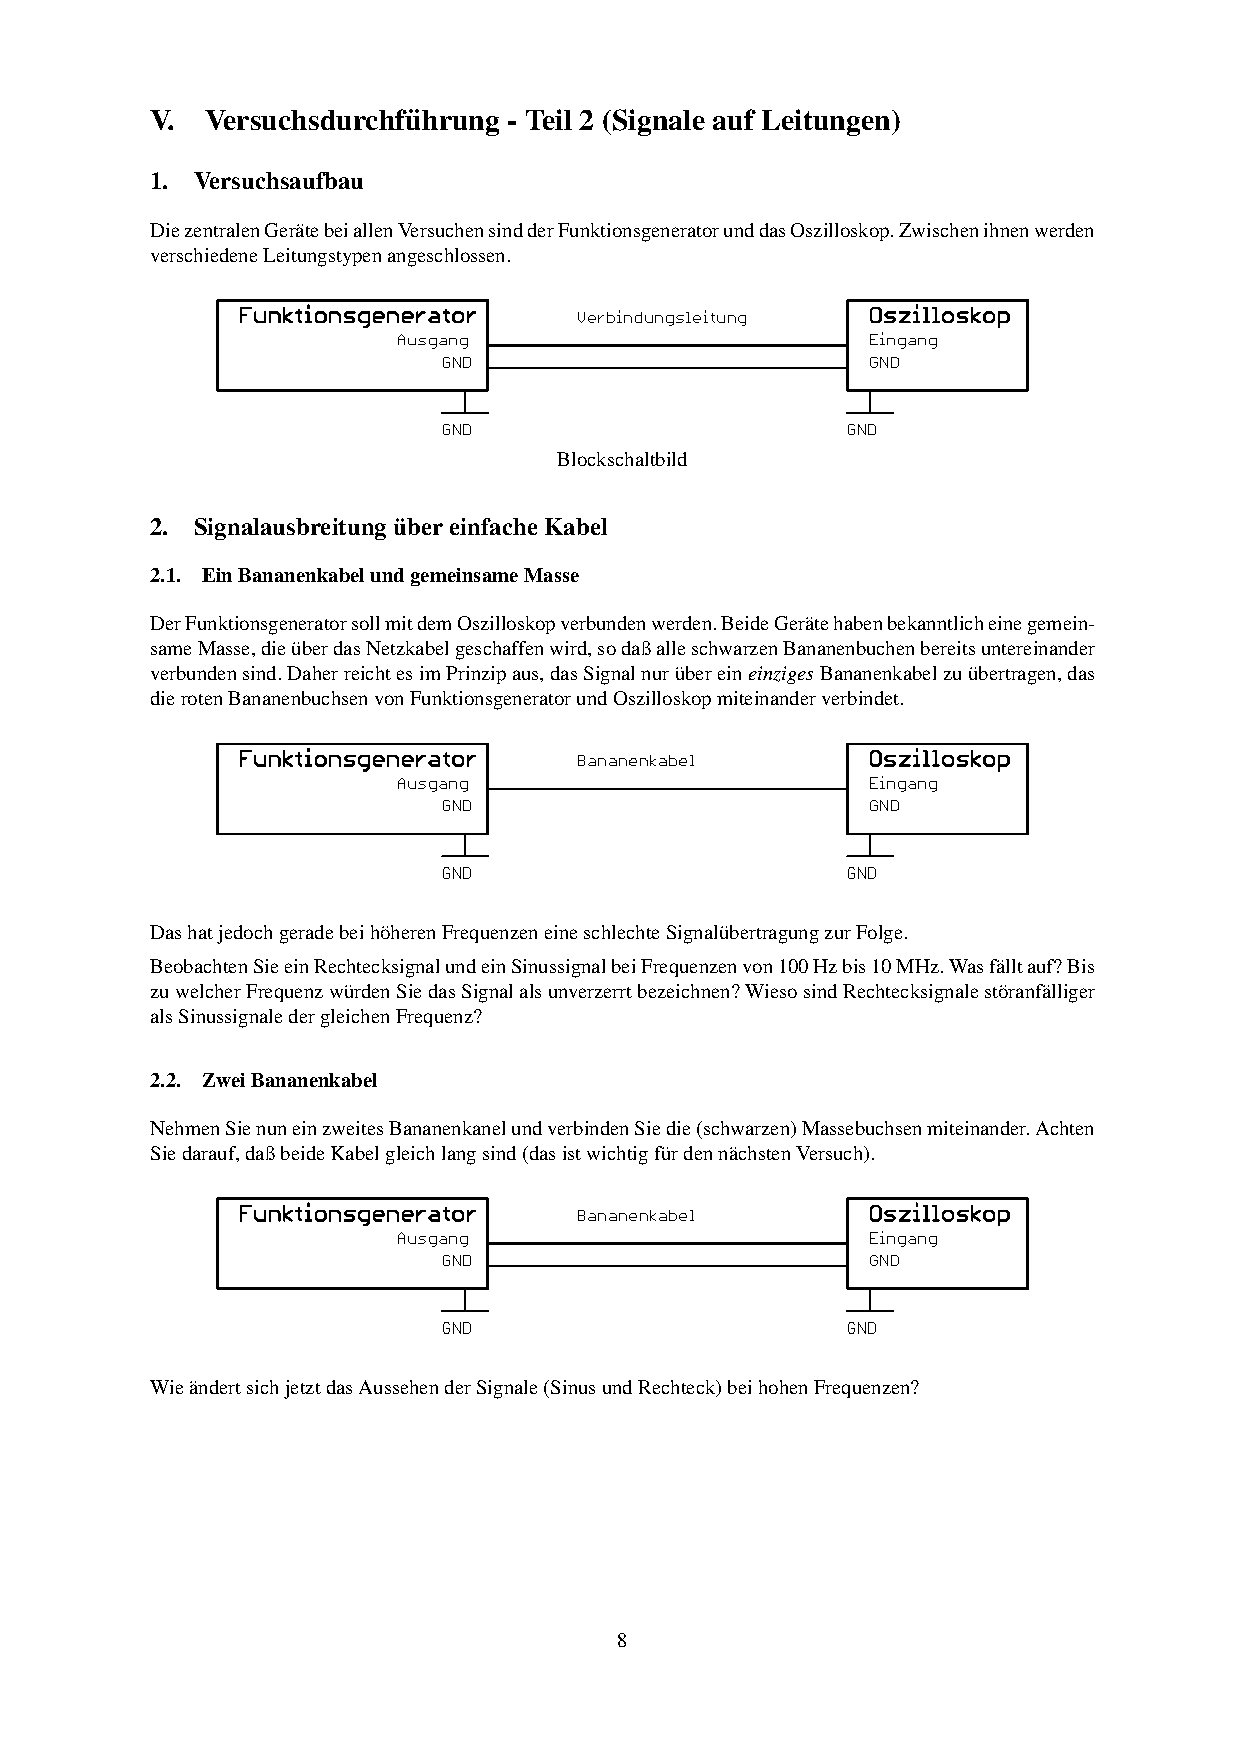
\includegraphics[trim = 10mm 210mm 10mm 50mm, clip, scale = 1]{2_0-2_2.pdf}
  	\caption[Schaltskizze einer Verbindung zwischen Funktionsgenerator und Oszilloskop]{Schaltskizze einer Verbindung zwischen Funktionsgenerator und Oszilloskop\footnotemark}
  \label{fig:2.0}
\end{figure}
\footnotetext{Abbildung entnommen von http://www.atlas.uni-wuppertal.de/$\sim$kind/ep1\_14.pdf Seite 8 am 19.10.2014}

\begin{figure}[H] 
  \centering
    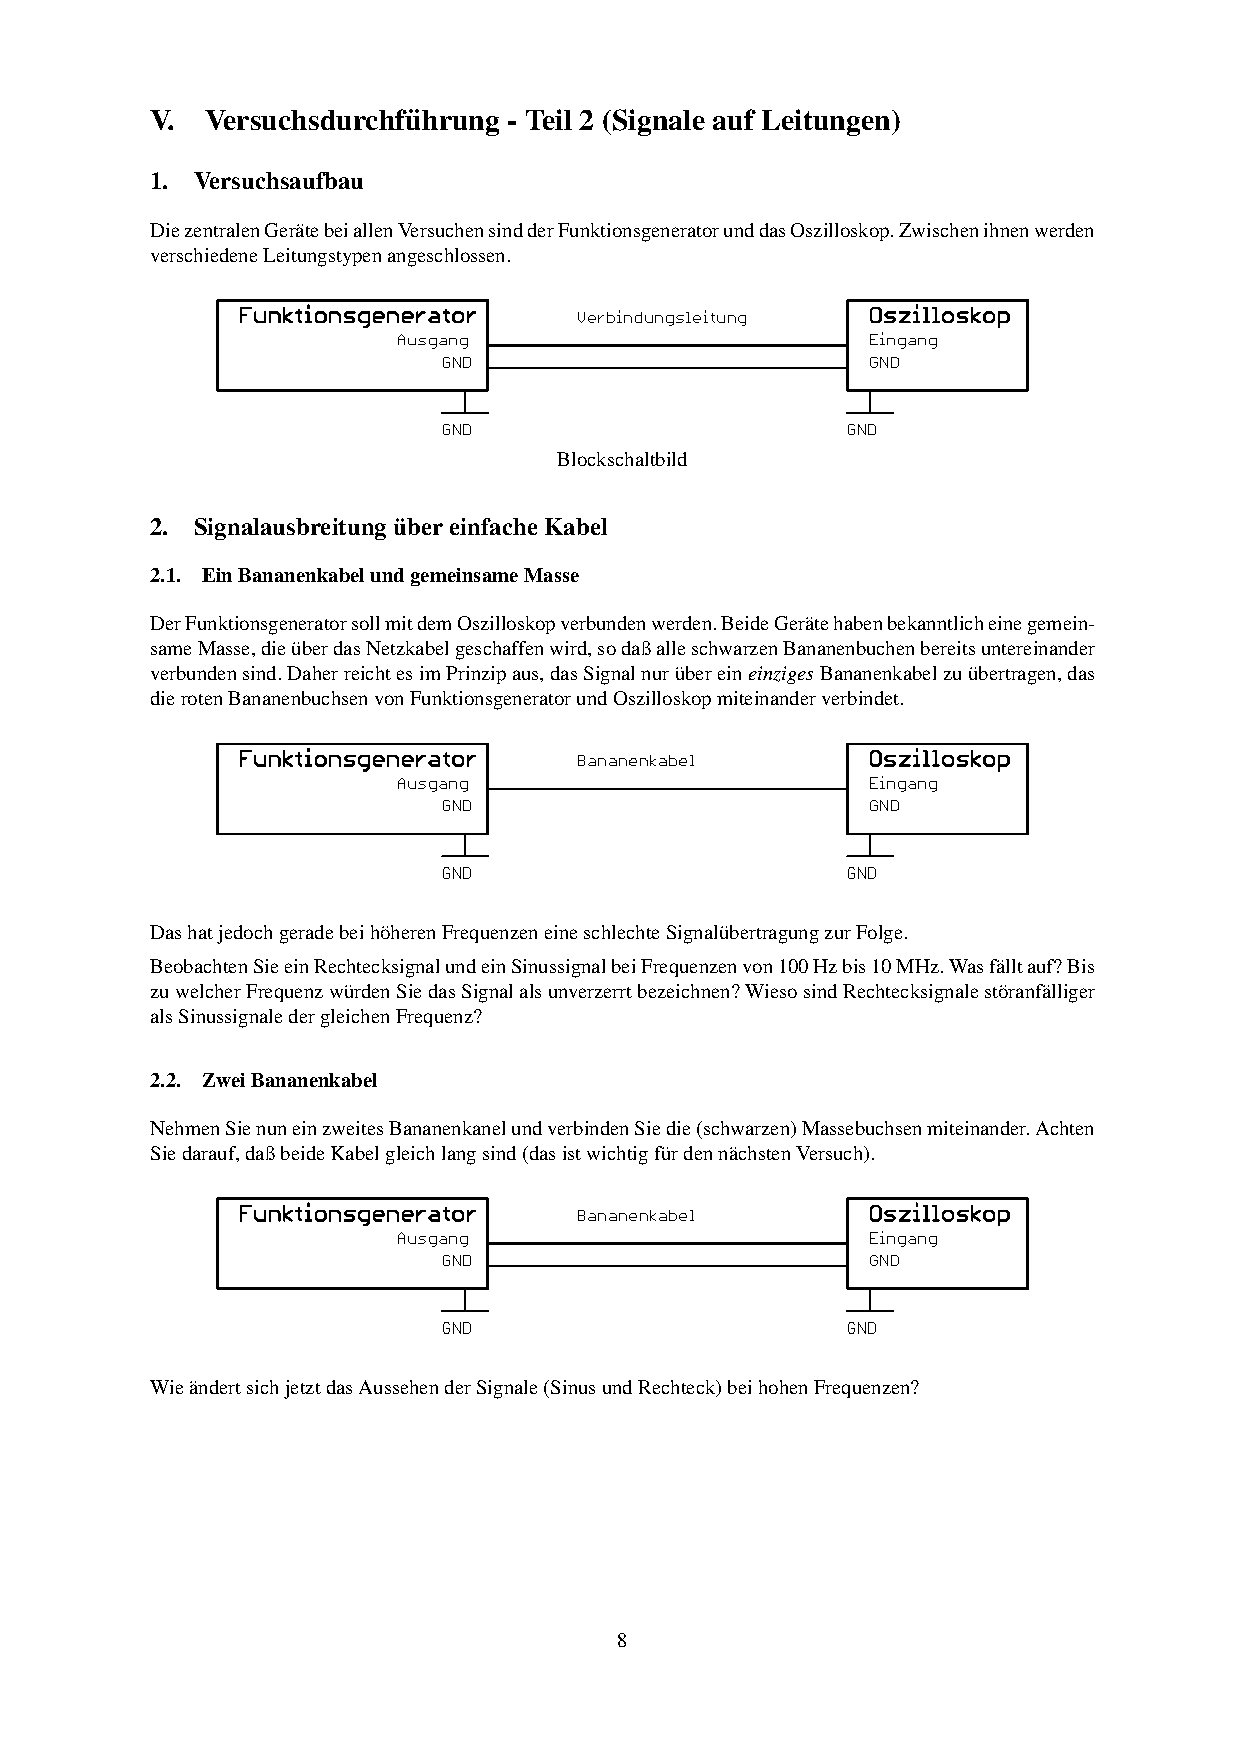
\includegraphics[trim = 10mm 142mm 10mm 125mm, clip, scale = 1]{2_0-2_2.pdf}
  	\caption[Schaltskizze einer Verbindung zwischen Funktionsgenerator und Oszilloskop, mit einem Bananenkabel]{Schaltskizze einer Verbindung zwischen Funktionsgenerator und Oszilloskop, mit einem Bananenkabel\footnotemark}
  \label{fig:2.1}
\end{figure}
\footnotetext{Abbildung entnommen von http://www.atlas.uni-wuppertal.de/$\sim$kind/ep1\_14.pdf Seite 8 am 19.10.2014}

\begin{figure}[H] 
  \centering
    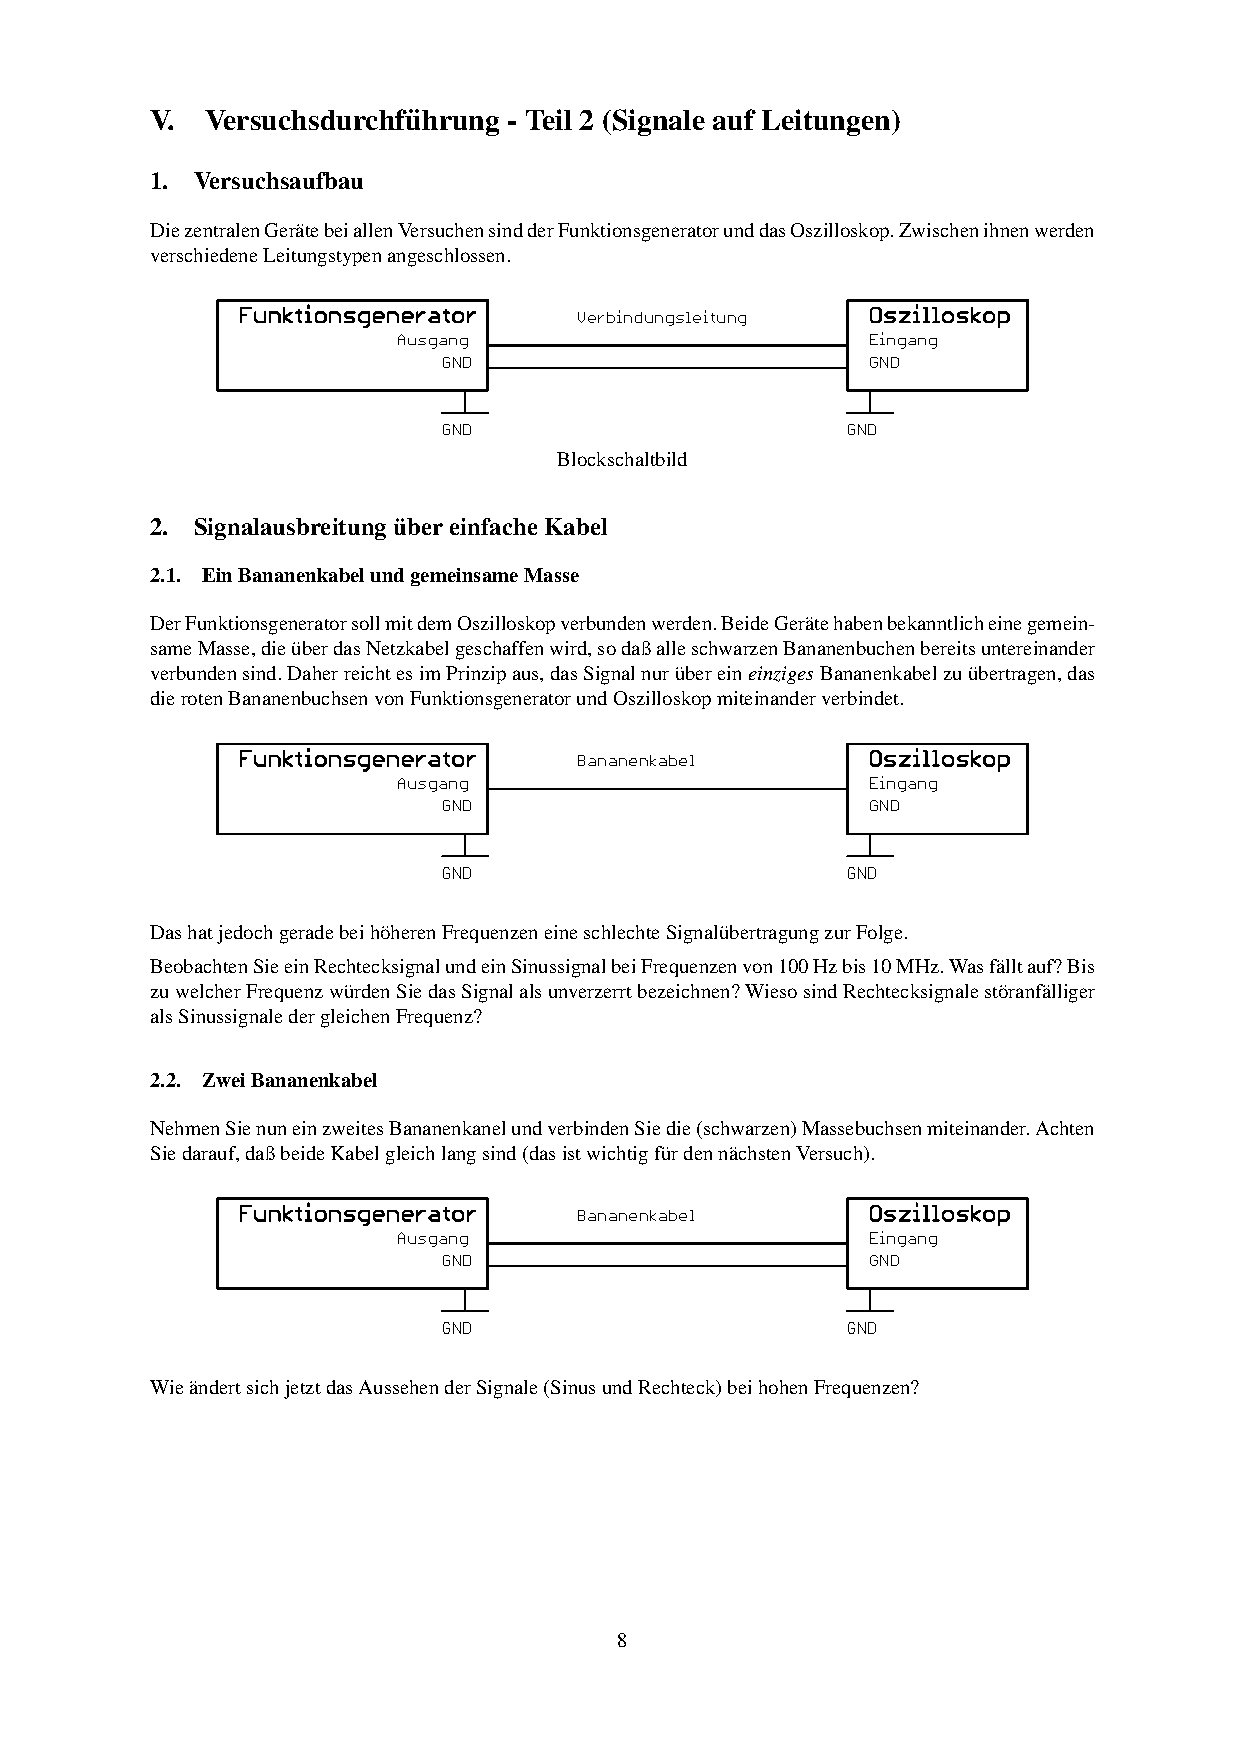
\includegraphics[trim = 10mm 70mm 10mm 200mm, clip, scale = 1]{2_0-2_2.pdf}
  	\caption[Schaltskizze einer Verbindung zwischen Funktionsgenerator und Oszilloskop, mit zwei Bananenkabeln]{Schaltskizze einer Verbindung zwischen Funktionsgenerator und Oszilloskop, mit zwei Bananenkabeln\footnotemark}
  \label{fig:2.2}
\end{figure}
\footnotetext{Abbildung entnommen von http://www.atlas.uni-wuppertal.de/$\sim$kind/ep1\_14.pdf Seite 8 am 19.10.2014}

\begin{figure}[H] 
  \centering
    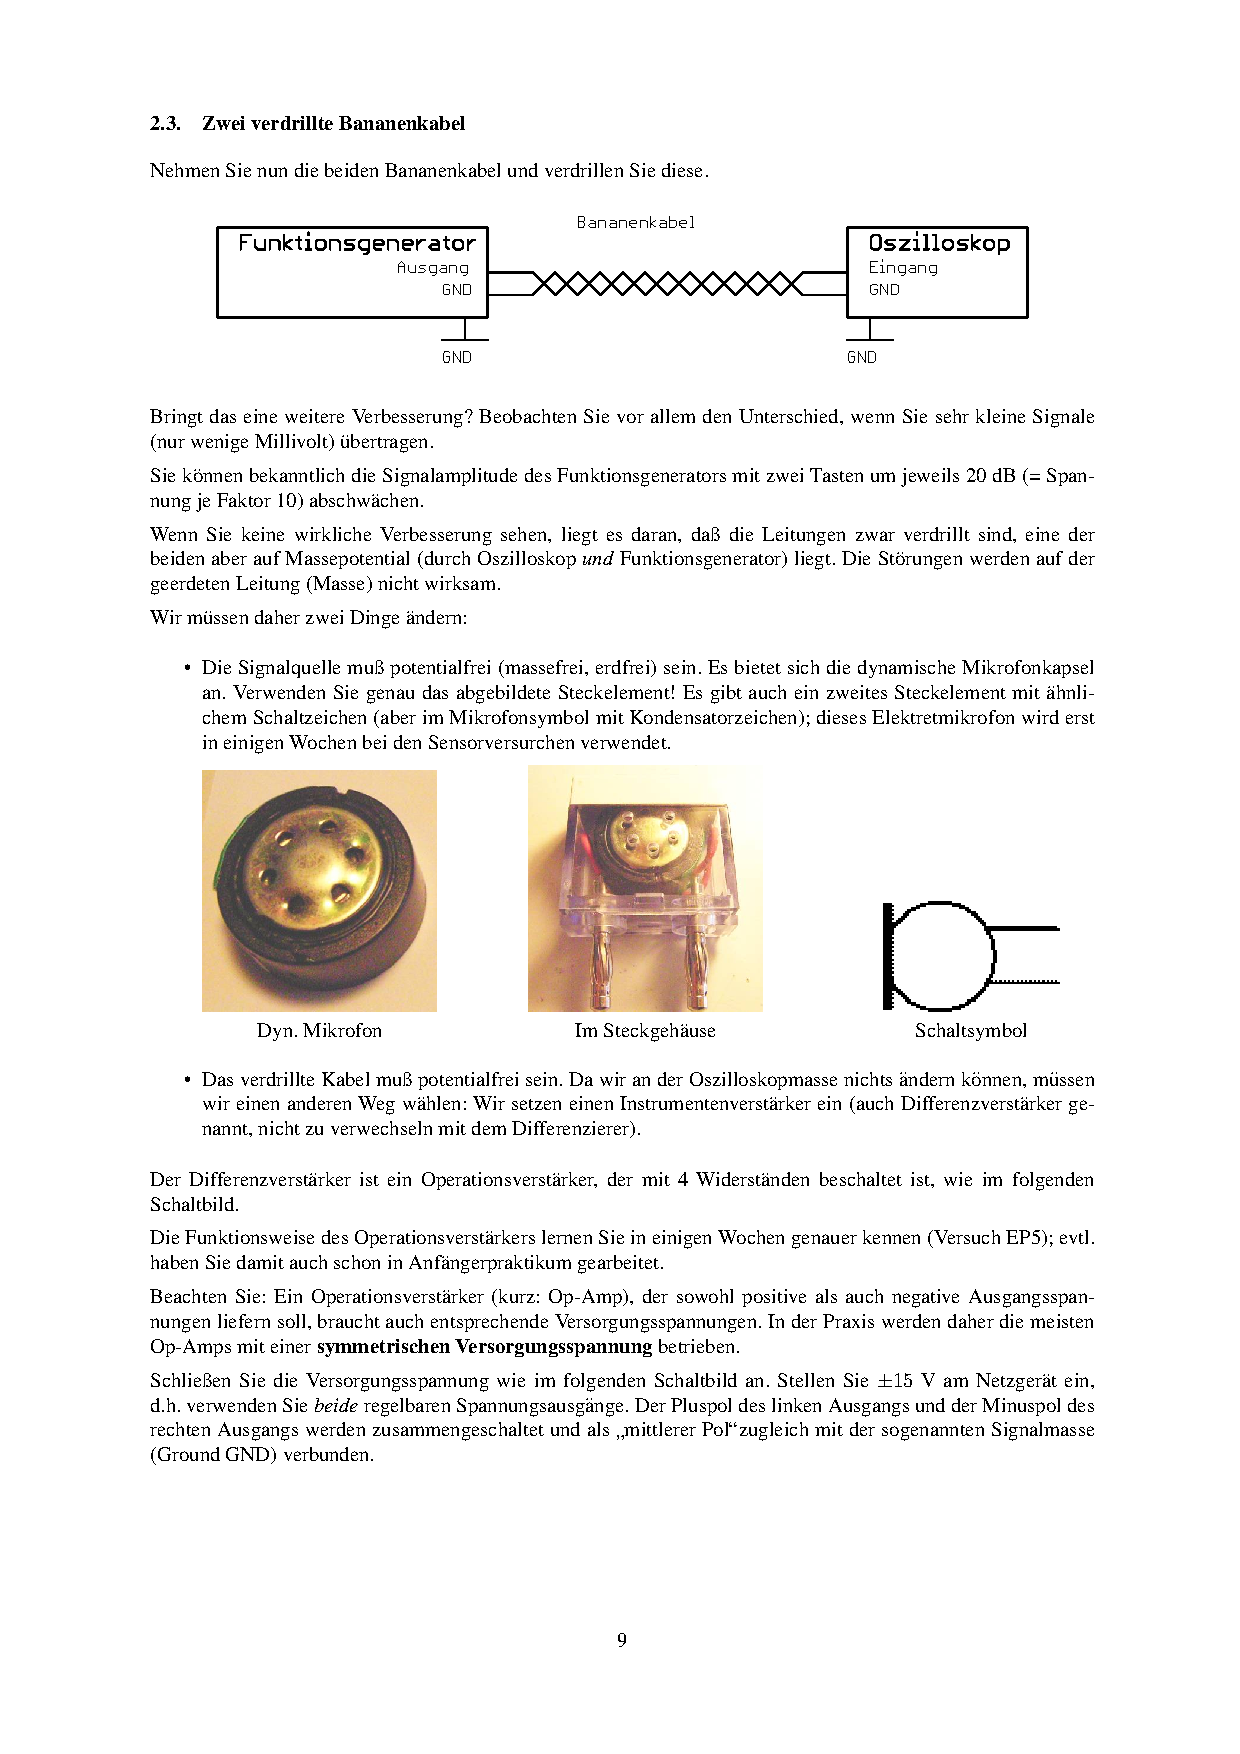
\includegraphics[trim = 10mm 230mm 10mm 32mm, clip, scale = 1]{2_3.pdf}
  	\caption[Schaltskizze einer Verbindung zwischen Funktionsgenerator und Oszilloskop, mit zwei verdrillten Bananenkabeln]{Schaltskizze einer Verbindung zwischen Funktionsgenerator und Oszilloskop, mit zwei verdrillten Bananenkabeln\footnotemark}
  \label{fig:2.3}
\end{figure}
\footnotetext{Abbildung entnommen von http://www.atlas.uni-wuppertal.de/$\sim$kind/ep1\_14.pdf Seite 9 am 19.10.2014}


\begin{figure}[H] 
  \centering
    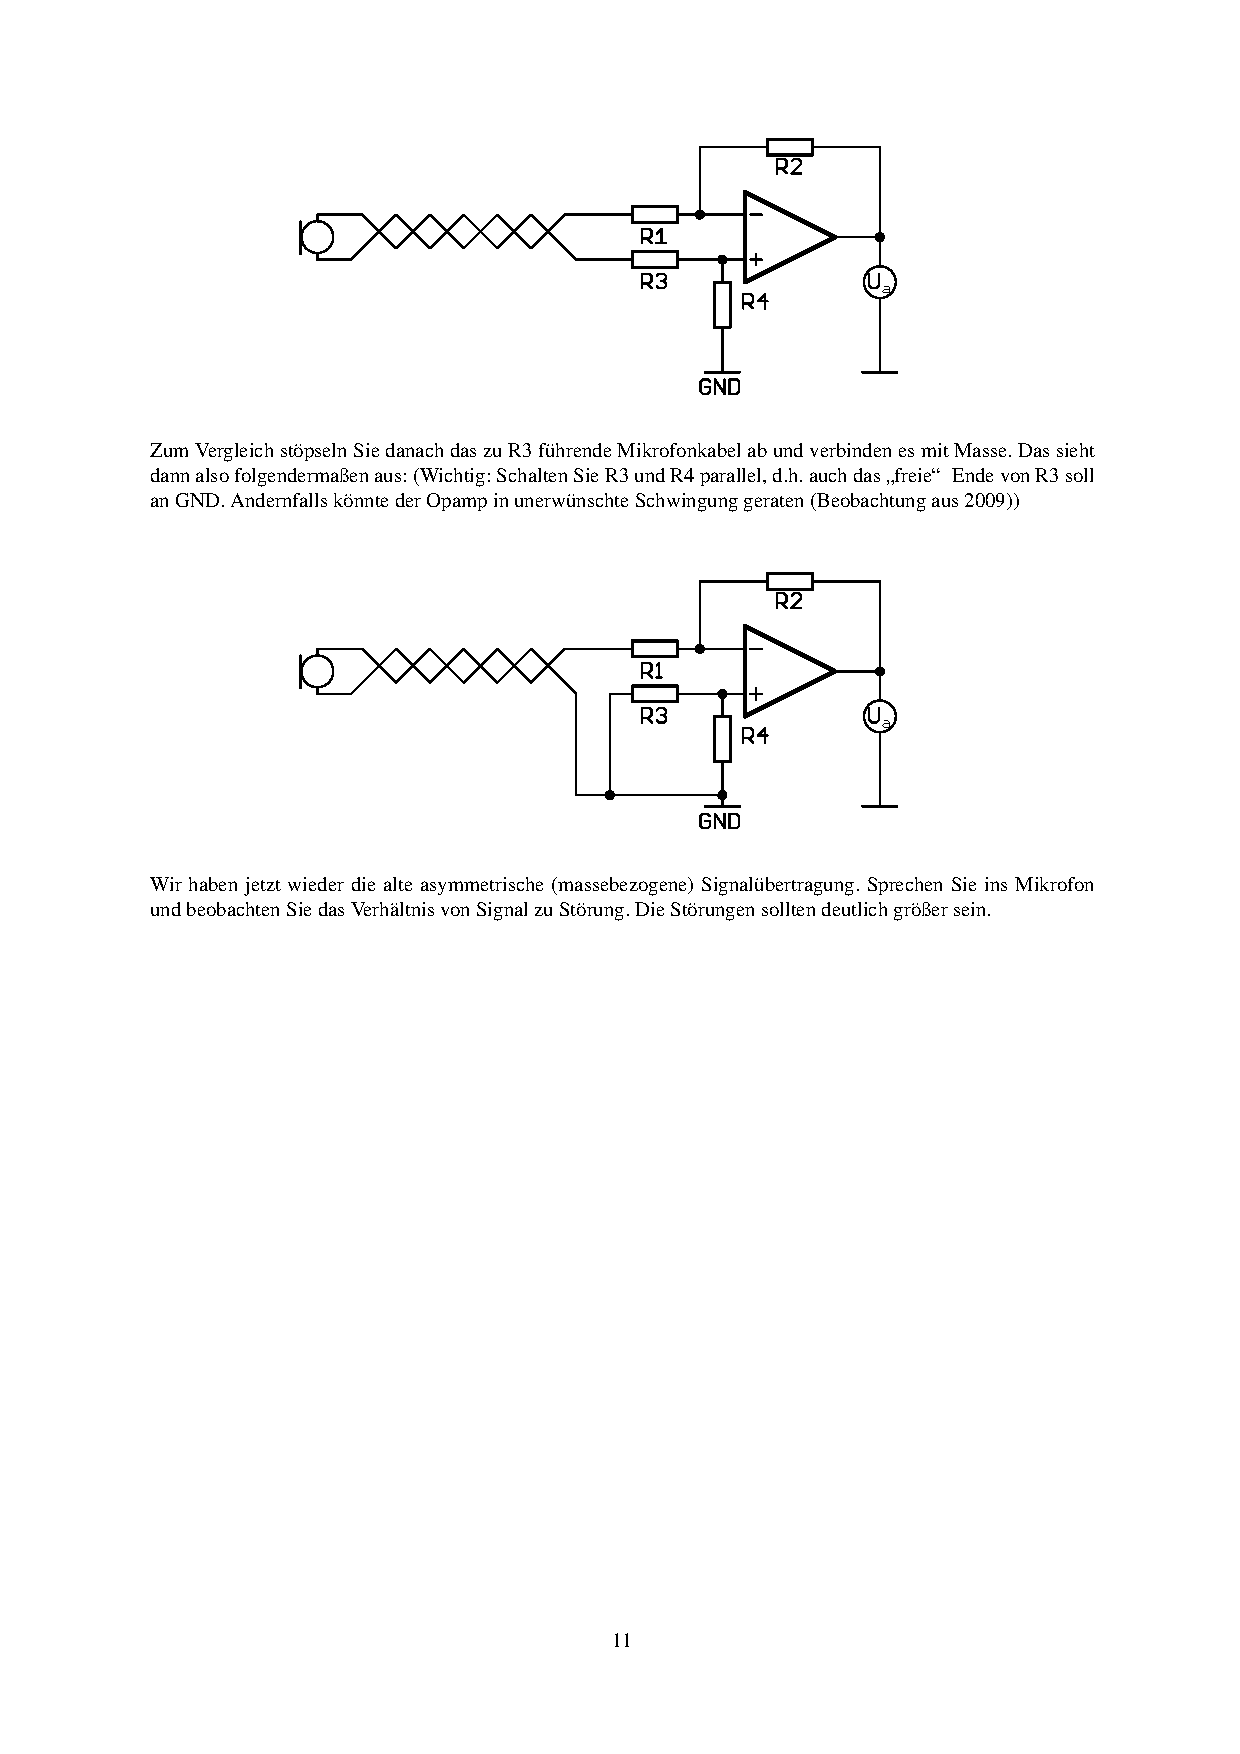
\includegraphics[trim = 10mm 230mm 10mm 20mm, clip, scale = 1]{2_3+Op-Amp.pdf}
  	\caption[Schaltskizze des Aufbaus mit Operationsverstärker und verdrillten Bananenkabeln]{Schaltskizze des Aufbaus mit Operationsverstärker und verdrillten Bananenkabeln\footnotemark}
  \label{fig:2.4}
\end{figure}
\footnotetext{Abbildung entnommen von http://www.atlas.uni-wuppertal.de/$\sim$kind/ep1\_14.pdf Seite 11 am 19.10.2014}

\begin{figure}[H] 
  \centering
    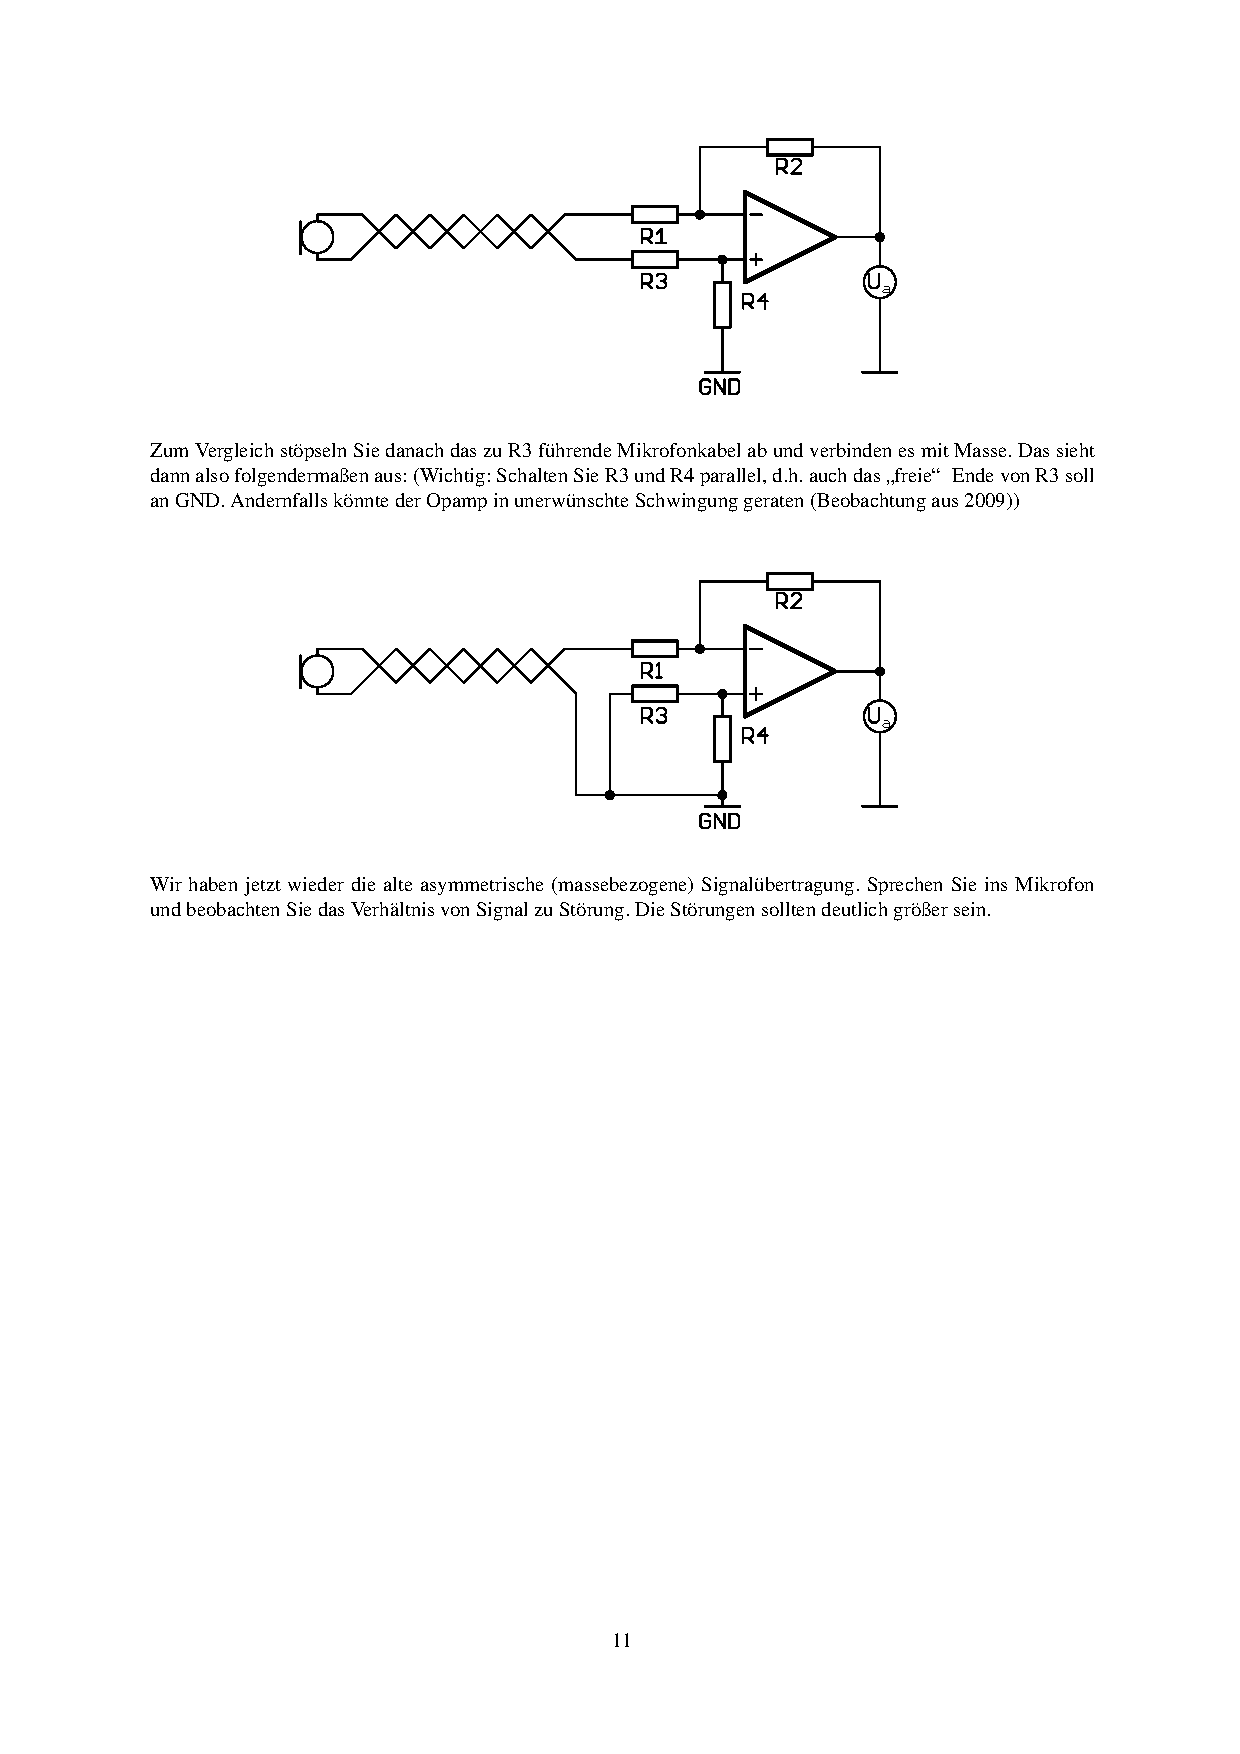
\includegraphics[trim = 10mm 160mm 10mm 90mm, clip, scale = 1]{2_3+Op-Amp.pdf}
  	\caption[Schaltskizze des Aufbaus mit Operationsverstärker und verdrillten Bananenkabeln, bei parallel geschaltetem R$_3$]{Schaltskizze des Aufbaus mit Operationsverstärker und verdrillten Bananenkabeln, bei parallel geschaltetem R$_3$\footnotemark}
  \label{fig:2.5}
\end{figure}
\footnotetext{Abbildung entnommen von http://www.atlas.uni-wuppertal.de/$\sim$kind/ep1\_14.pdf Seite 11 am 19.10.2014}


\begin{figure}[H] 
  \centering
    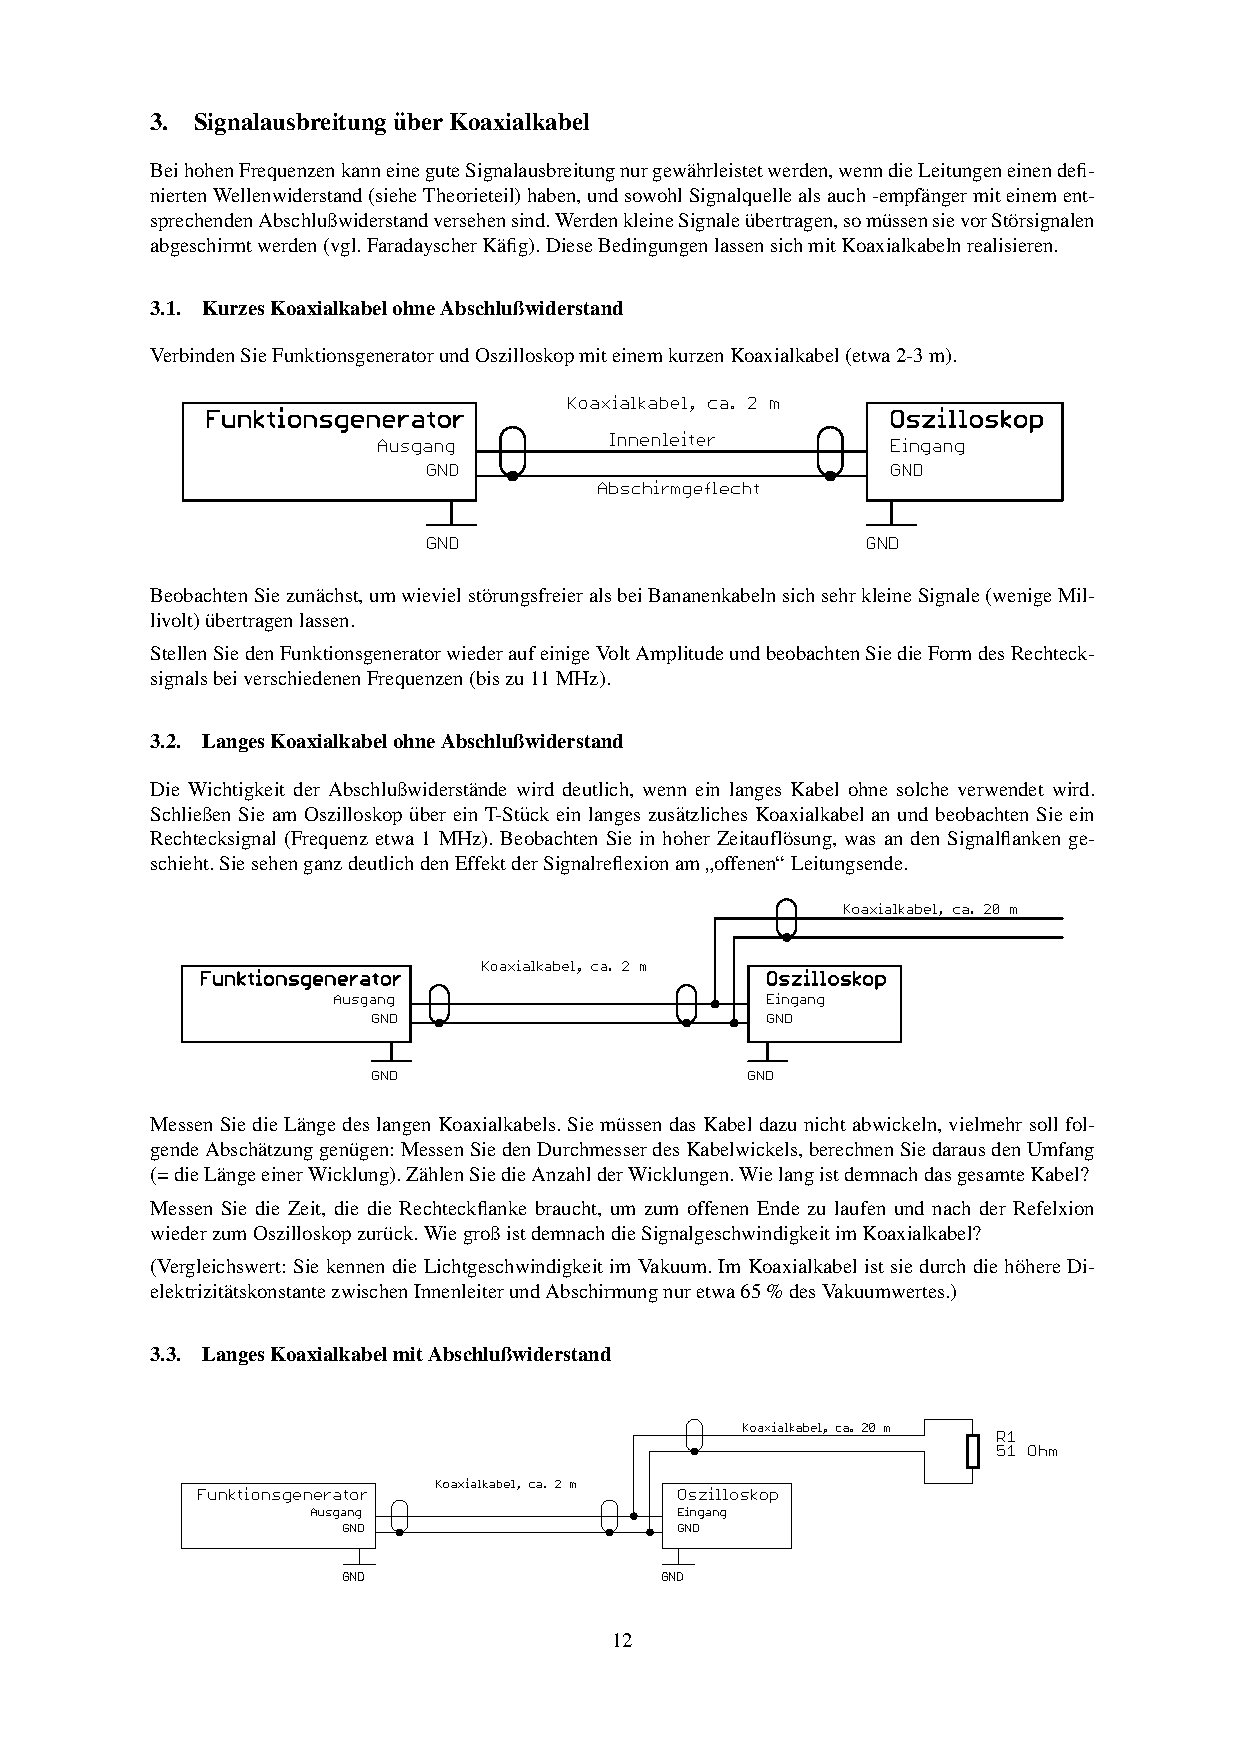
\includegraphics[trim = 10mm 200mm 10mm 65mm, clip, scale = 1]{3-3_3.pdf}
  	\caption[Schaltskizze einer Verbindung zwischen Funktionsgenerator und Oszilloskop, mit kurzem Koaxialkabel]{Schaltskizze einer Verbindung zwischen Funktionsgenerator und Oszilloskop, mit kurzem Koaxialkabel\footnotemark}
  \label{fig:3.1}
\end{figure}
\footnotetext{Abbildung entnommen von http://www.atlas.uni-wuppertal.de/$\sim$kind/ep1\_14.pdf Seite 12 am 19.10.2014}

\begin{figure}[H] 
  \centering
    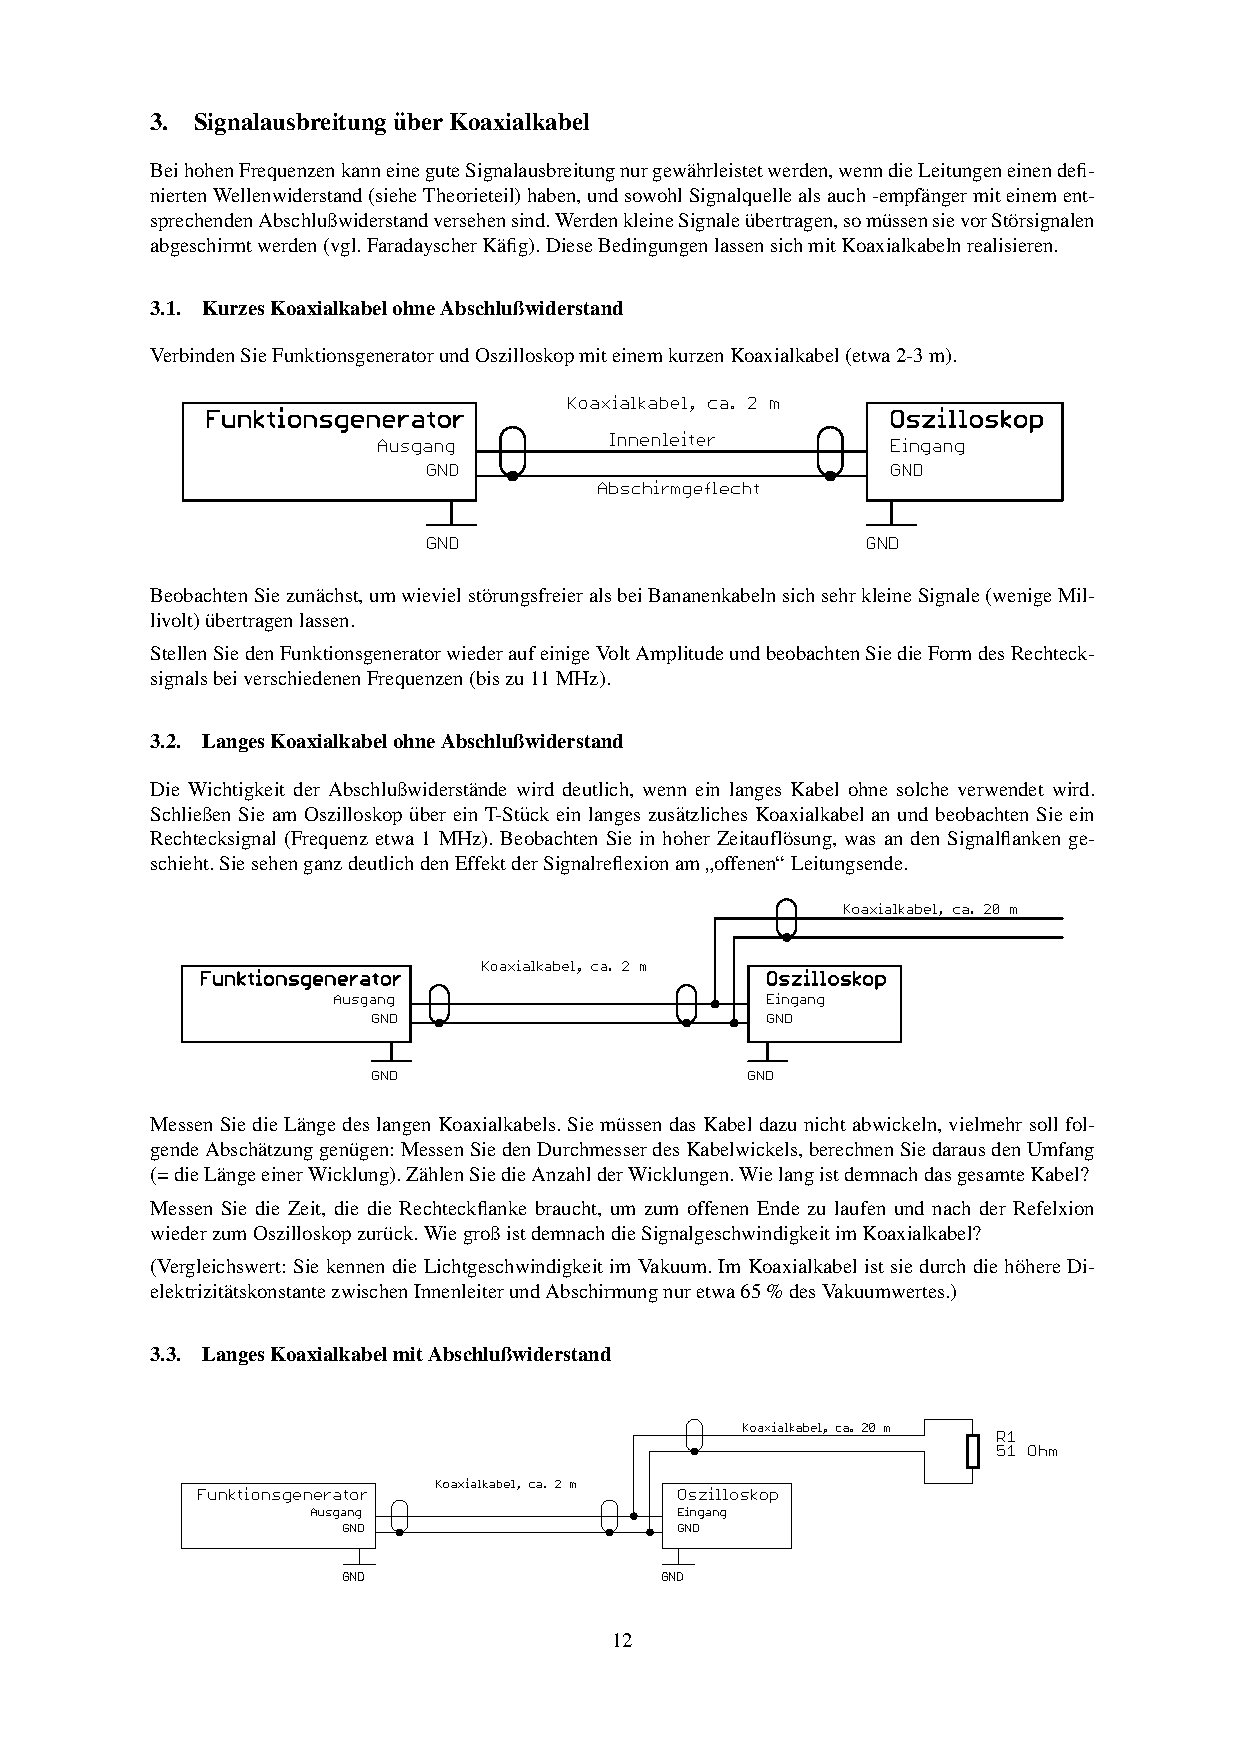
\includegraphics[trim = 10mm 110mm 10mm 150mm, clip, scale = 1]{3-3_3.pdf}
  	\caption[Schaltskizze einer Verbindung zwischen Funktionsgenerator und Oszilloskop, mit langem Koaxialkabel]{Schaltskizze einer Verbindung zwischen Funktionsgenerator und Oszilloskop, mit langem Koaxialkabel\footnotemark}
  \label{fig:3.2}
\end{figure}
\footnotetext{Abbildung entnommen von http://www.atlas.uni-wuppertal.de/$\sim$kind/ep1\_14.pdf Seite 12 am 19.10.2014}


\begin{figure}[H] 
  \centering
    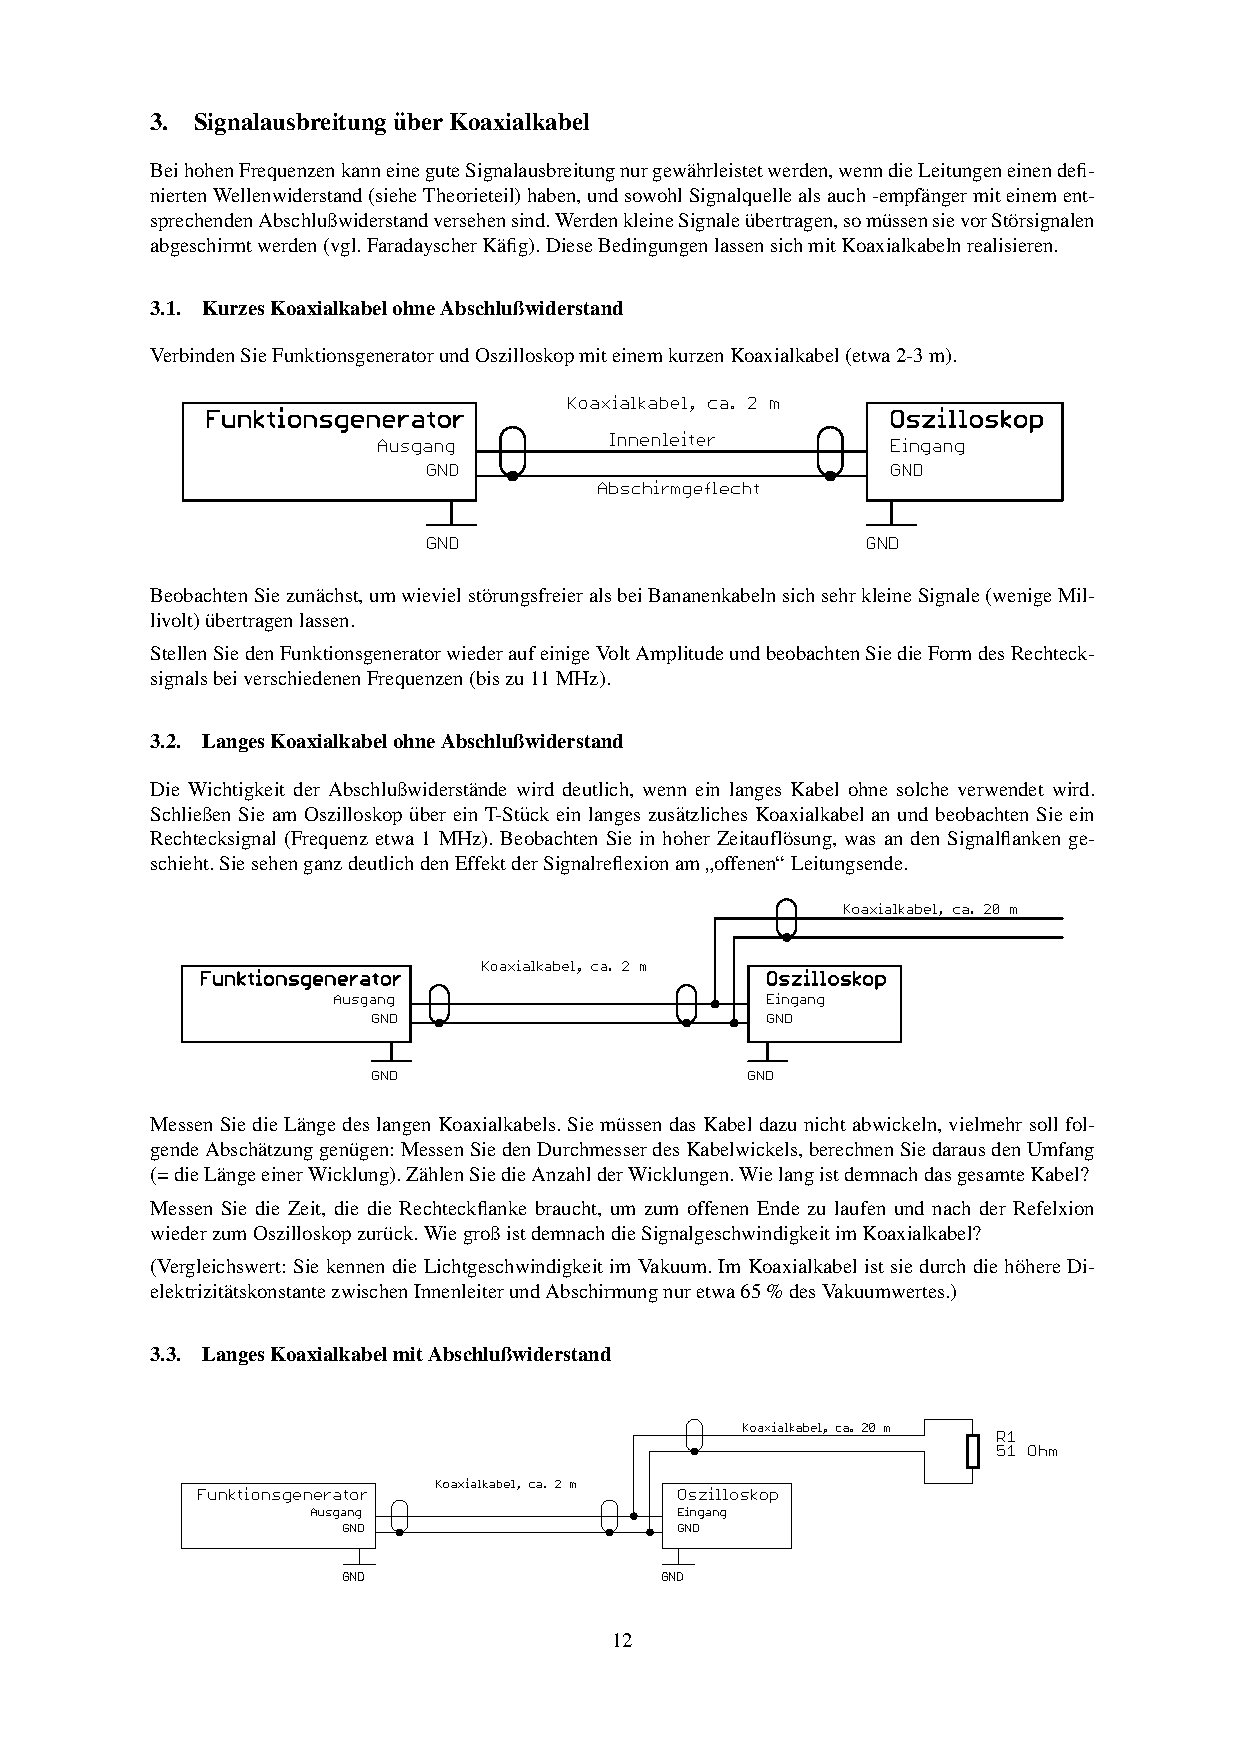
\includegraphics[trim = 10mm 25mm 10mm 235mm, clip, scale = 1]{3-3_3.pdf}
  	\caption[Schaltskizze einer Verbindung zwischen Funktionsgenerator und Oszilloskop, mit langem Koaxialkabel und Abschlusskabel]{Schaltskizze einer Verbindung zwischen Funktionsgenerator und Oszilloskop, mit langem Koaxialkabel und Abschlusskabel\footnotemark}
  \label{fig:3.3}
\end{figure}
\footnotetext{Abbildung entnommen von http://www.atlas.uni-wuppertal.de/$\sim$kind/ep1\_14.pdf Seite 12 am 19.10.2014}


\begin{figure}[H] 
  \centering
    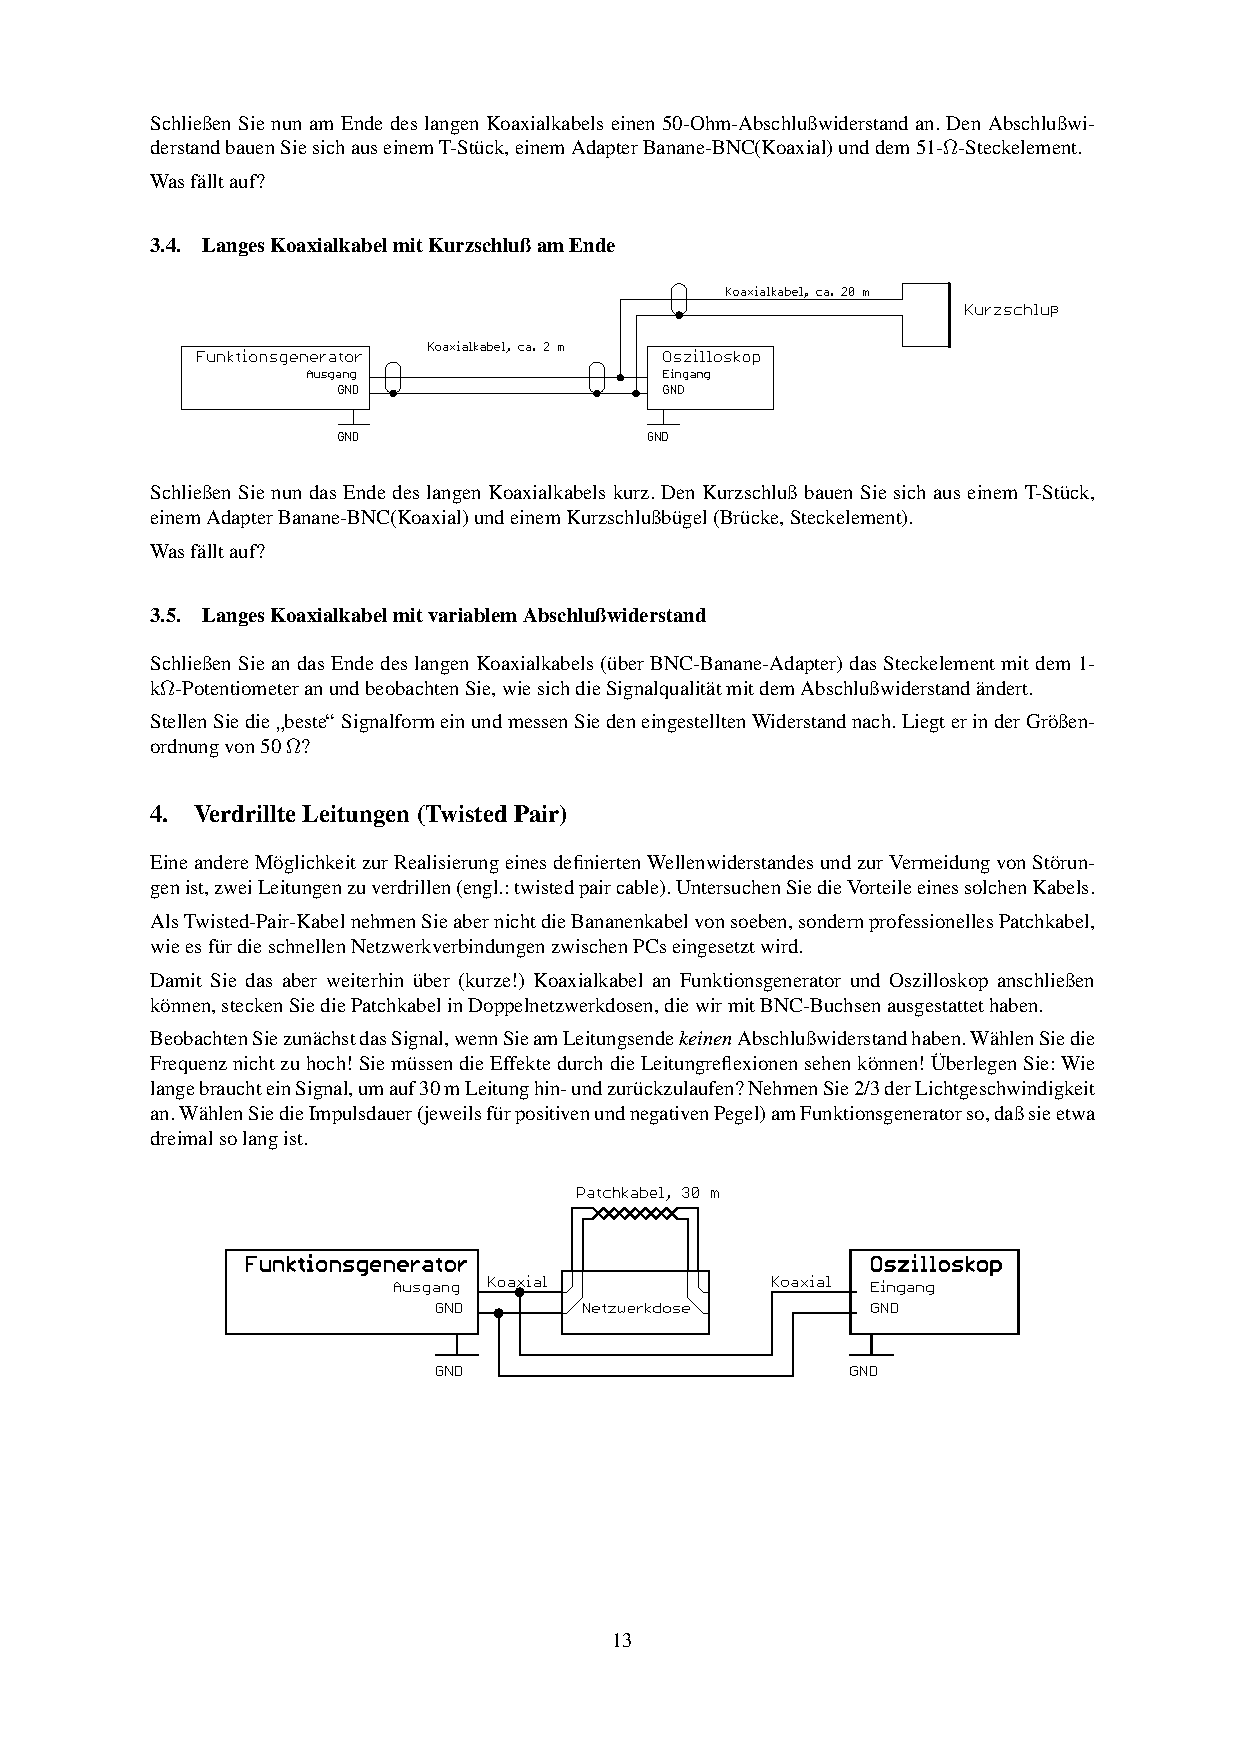
\includegraphics[trim = 10mm 220mm 10mm 45mm, clip, scale = 1]{3_4-4.pdf}
  	\caption[Schaltskizze einer Verbindung zwischen Funktionsgenerator und Oszilloskop, mit langem Koaxialkabel und Kurzschluss]{Schaltskizze einer Verbindung zwischen Funktionsgenerator und Oszilloskop, mit langem Koaxialkabel und Kurzschluss\footnotemark}
  \label{fig:3.4}
\end{figure}
\footnotetext{Abbildung entnommen von http://www.atlas.uni-wuppertal.de/$\sim$kind/ep1\_14.pdf Seite 13 am 19.10.2014}


\begin{figure}[H] 
  \centering
    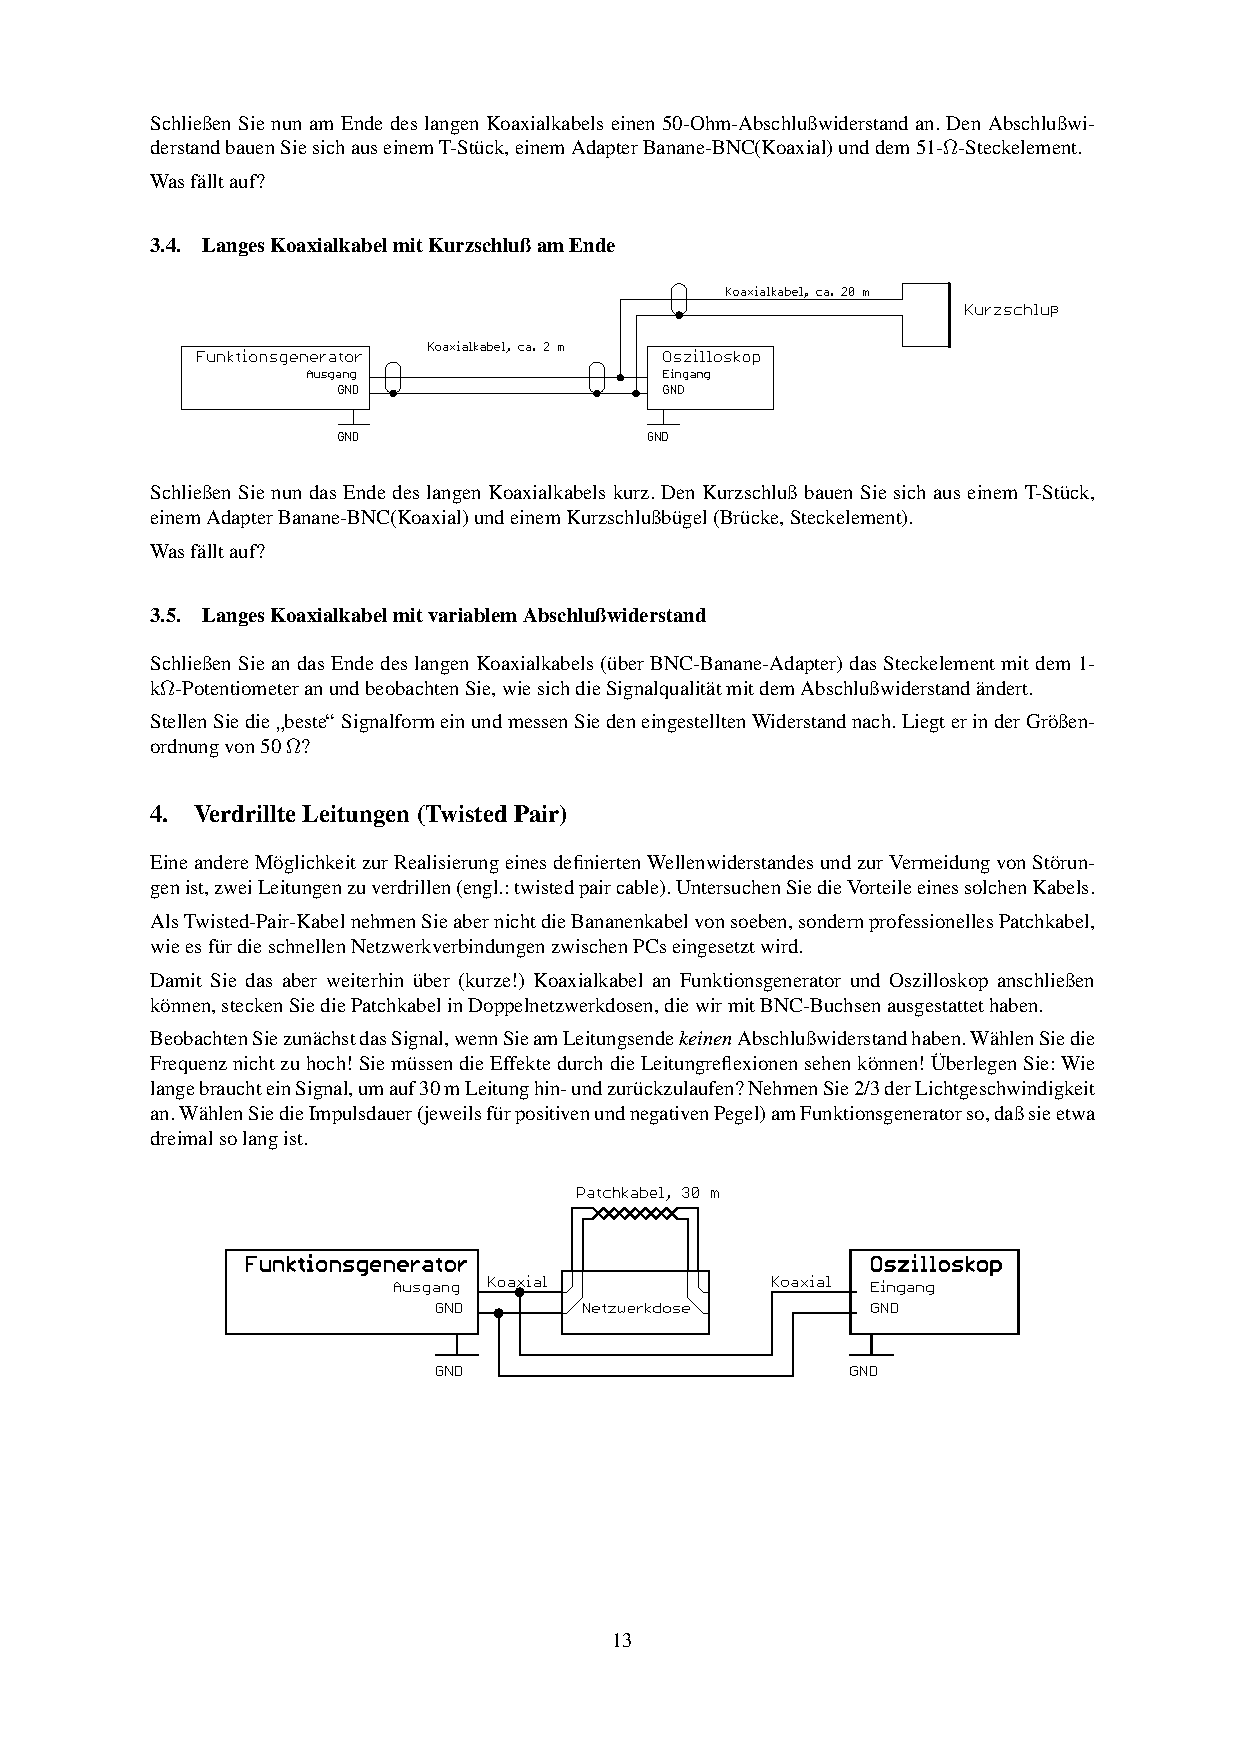
\includegraphics[trim = 10mm 60mm 10mm 200mm, clip, scale = 1]{3_4-4.pdf}
  	\caption[Schaltskizze einer Verbindung zwischen Funktionsgenerator und Oszilloskop, mit Patch- und Koaxialkabel]{Schaltskizze einer Verbindung zwischen Funktionsgenerator und Oszilloskop, mit Patch- und Koaxialkabel\footnotemark}
  \label{fig:4.1}
\end{figure}
\footnotetext{Abbildung entnommen von http://www.atlas.uni-wuppertal.de/$\sim$kind/ep1\_14.pdf Seite 14 am 19.10.2014}


\begin{figure}[H] 
  \centering
    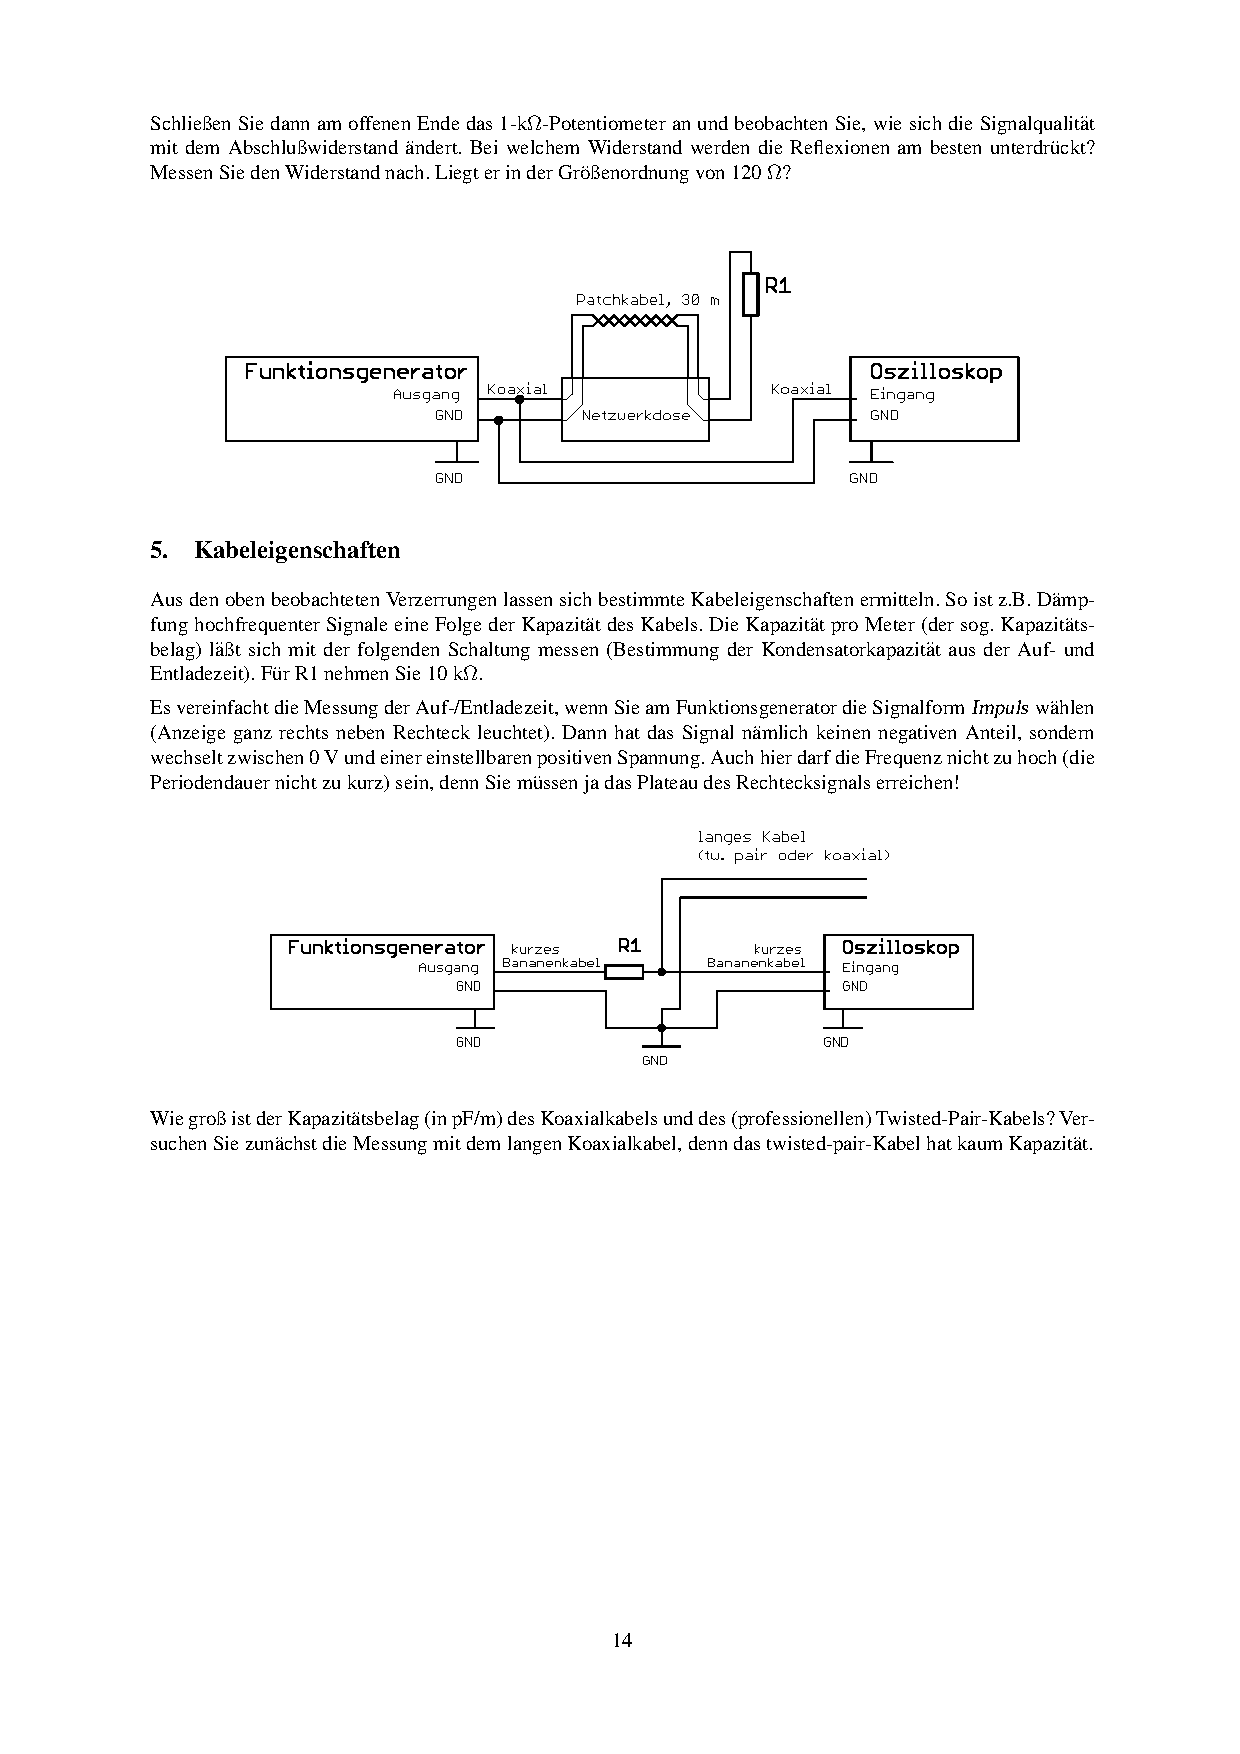
\includegraphics[trim = 10mm 210mm 10mm 40mm, clip, scale = 1]{4-5.pdf}
  	\caption[Schaltskizze einer Verbindung zwischen Funktionsgenerator und Oszilloskop, mit Patch- und Koaxialkabel (geschlossen mit Potentiometer)]{Schaltskizze einer Verbindung zwischen Funktionsgenerator und Oszilloskop, mit Patch- und Koaxialkabel (geschlossen mit Potentiometer)\footnotemark}
  \label{fig:4.2}
\end{figure}
\footnotetext{Abbildung entnommen von http://www.atlas.uni-wuppertal.de/$\sim$kind/ep1\_14.pdf Seite 14 am 19.10.2014}


\begin{figure}[H] 
  \centering
    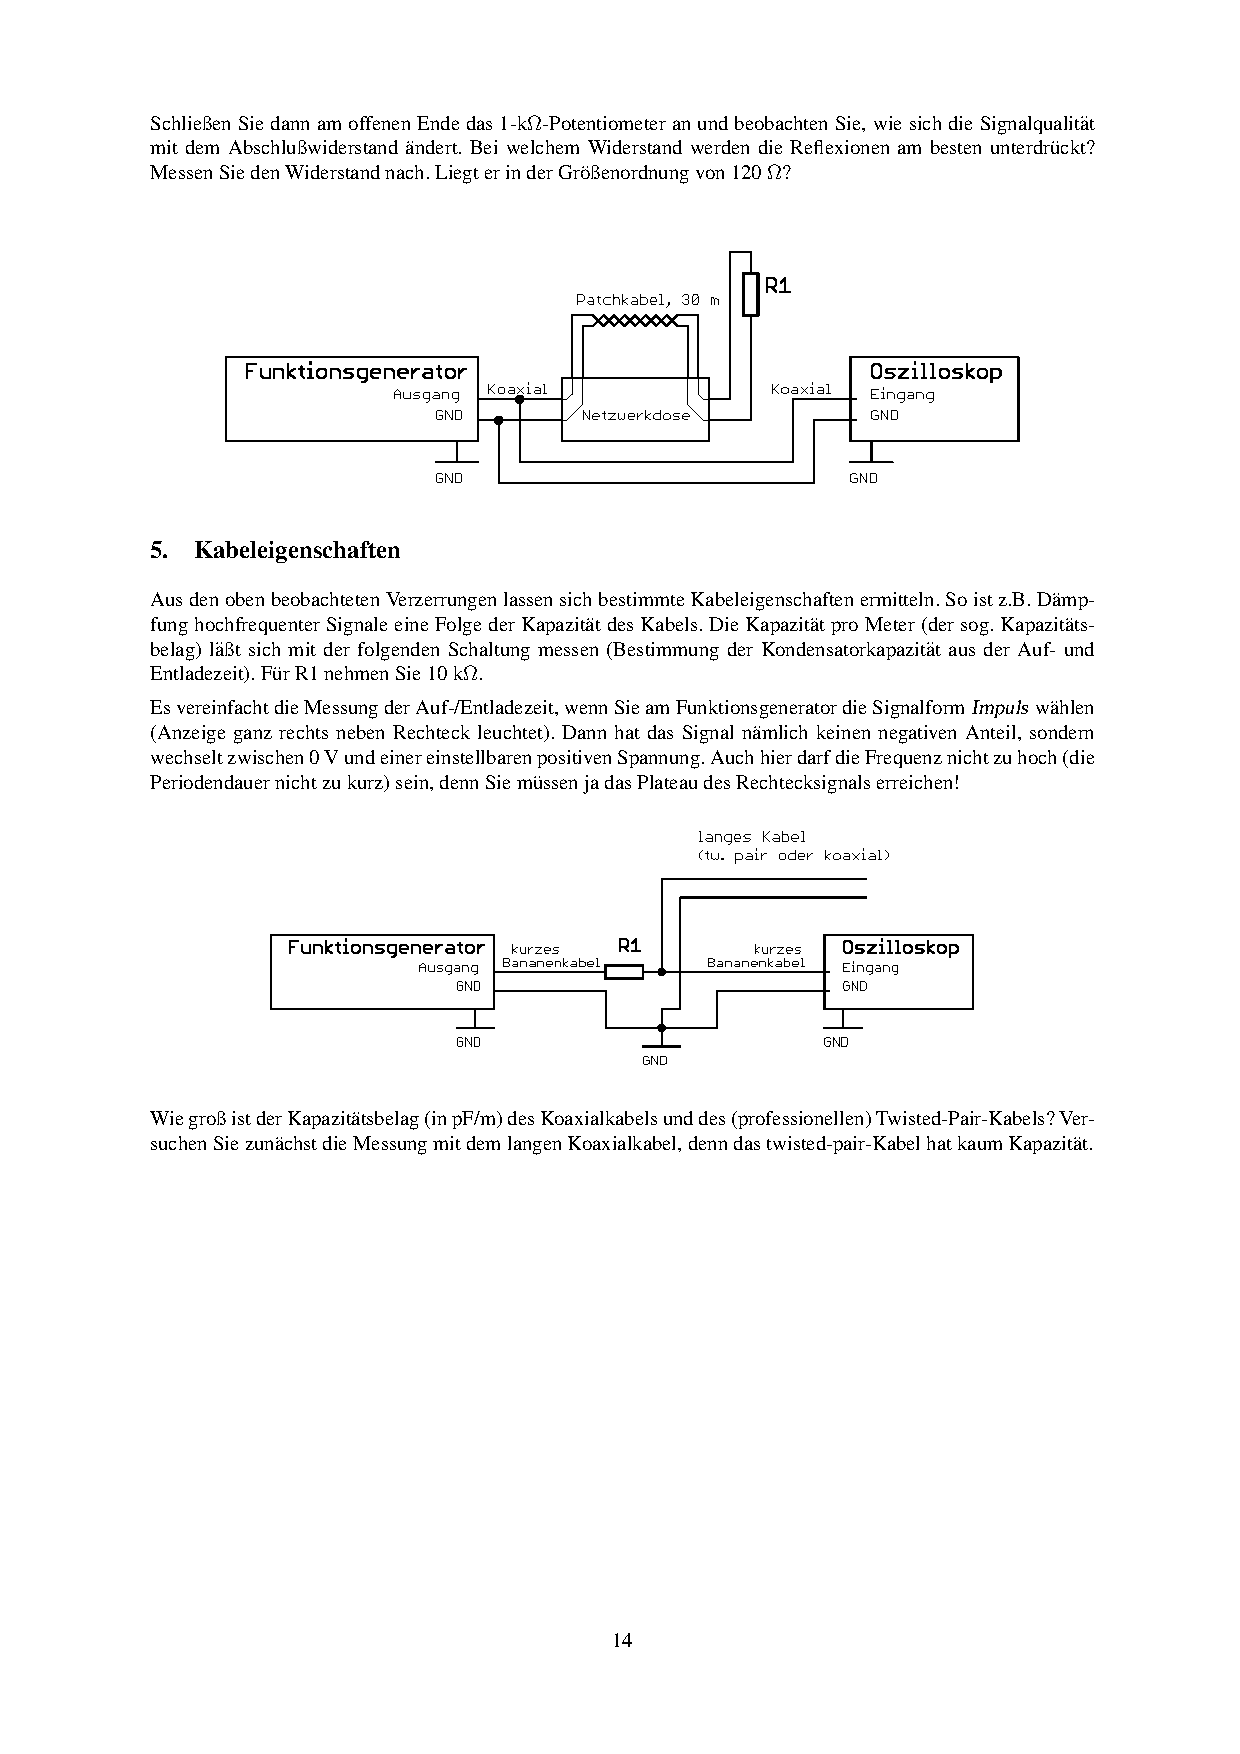
\includegraphics[trim = 10mm 110mm 10mm 140mm, clip, scale = 1]{4-5.pdf}
  	\caption[Schaltskizze zur Bestimmung des Kapazitätsbelags]{Schaltskizze zur Bestimmung des Kapazitätsbelags\footnotemark}
  \label{fig:5}
\end{figure}
\footnotetext{Abbildung entnommen von http://www.atlas.uni-wuppertal.de/$\sim$kind/ep1\_14.pdf Seite 14 am 19.10.2014}

\newpage\section{Einleitung}
%einleitung zu dem experiment.
%auf die einstellungen, die vor dem versuch gemacht werden, eingehen oder auf eine anleitung dazu verweisen.
%---------------------------------------------------------------------------------------------
%hinter der einleitung kann der allgemeine theoretische hintergrund in einer zusätzlichen section erklärt werden

\section{Verwendete Materialien}
%(immer) eine skizze oder ein foto einfügen, die geräte/materialien !nummerieren! und z.b. eine legende dazu schreiben
%falls am anfang des versuches nicht klar ist, was alles verwendet wird, wenn möglich erst am ende ein großes foto von den verwendeten materialien machen!
%-------------------------------------------------------------------------------------------
%ab hier für jeden versuchsteil einzeln, falls noch materialien hinzugenommen wurden immer im versuchsaufbau erwähnen!
\section{Versuchsteil...}
%kurz das ziel dieses versuchsteiles ansprechen, damit keine zwei überschriften direkt übereinander stehen!
%bei schwierigeren versuchen kann auch der theoretische hintergrund erläutert werden. (mit formeln, herleitungen und erklärungen)
\subsection{Versuchsaufbau}
%skizze zum versuchsaufbau (oder foto) einfügen,   es muss erklärt werden wie das ganze funktioniert und welche speziellen einstellungen verwendet wurden (z.b. welche knöpfe an den geräten für die messung verdreht wurden)
\subsection{Versuchsdurchführung}
%erklären, !was! wir machen, !warum! wir das machen und mit welchem ziel
%(wichtig) präzize erklären, wie bei dem versuch vorgegangen und was gemacht wurde
\subsection{Verwendete Formeln}
%eine legende kann angefertigt werden, die selbstverständlichen buchstaben müssen nicht extra erklärt werden
%mit knappen erklärungen die !verwendeten! formeln, sowie die zugehörige fehlerrechnung einfügen.
\subsection{Messergebnisse}
%die messwerte in !übersichtlichen! tabellen angegeben
%zu viele kleine tabellen in große tabellen überführen!
%zu große tabellen mit dem [scale]-befehl scalieren oder (falls zu lang) in zwei kleinere tabellen aufteilen
%(wichtig) vor !jeder! tabelle sagen, was gemessen wurde und wie die fehler gewählt wurden und ausreichend !erklären!, !warum! wir unsere fehler grade so gewählt haben
\subsection{Auswertung}
%zuerst !alle! errechneten werte entweder in ganzen sätzen aufzählen, oder in tabellen (übersichtlicher) dargestellen, sowie auf die verwendeten formeln verweisen (die referenzierung der formel kann in der überschrift stehen)
%kurz erwähnen (vor der tabelle), warum wir das ganze ausrechnen bzw. was wir dort ausrechnen
%danach histogramme und plots erstellen, wobei wenn möglich funktionen durch die plots gelegt werden (zur not können auch splines benutzt werden, was aber angegeben werden muss)
%bei fits immer die funktion und das reduzierte chiquadrat mit angegeben, wobei auf verständlichkeit beim entziffern der zehnerpotenzen geachtet werden muss z.b. f(x)=(wert+-fehler)\cdot10^{irgendeine zahl}\cdot x + (wert+-fehler)\cdot10^{irgendeine zahl}
%bei jedem fit erklären, nach welchem zusammenhang gefittet wurde und warum!
%bei plots darauf achten, dass die achsenbeschriftung (auch die tics) die richtige größe haben und die legende im plot nicht die messwerte verdeckt
%kurz die aufgabenstellung abgehandeln
\subsection{Diskussion}
%(immer) die gemessenen werte und die bestimmten werte über die messfehler mit literaturwerten oder untereinander vergleichen
%in welchem fehlerintervall des messwertes liegt der literaturwert oder der vergleichswert?
%wie ist der relative anteil des fehlers am messwert und damit die qualität unserer messung?
%in einem satz erklären, wie gut unser fehler und damit unsere messung ist
%kurz erläutern, wie systematische fehler unsere messung beeinflusst haben könnten
%(wichtig) zum schluss ansprechen, in wie weit die ergebnisse mit der theoretischen vorhersage übereinstimmen
%--------------------------------------------------------------------------------------------
%falls tabellen mit den messwerten zu lang werden, kann die section mit den messwerten auch hinter der diskussion angefügt bzw. eine section mit dem anhang eingefügt werden.
\section{Fazit}
%im fazit nochmal alles zusammenfassen und den verlauf der messung abschätzen
%gravierende sytematische probleme bei den messungen nochmal betonen und die wertigkeit unserer ergebnisse einordnen




\section{Versuchsteil 2}
%kurz das ziel dieses versuchsteiles ansprechen, damit keine zwei überschriften direkt übereinander stehen!
%bei schwierigeren versuchen kann auch der theoretische hintergrund erläutert werden. (mit formeln, herleitungen und erklärungen)
\subsection{Versuchsaufbau}
%skizze zum versuchsaufbau (oder foto) einfügen,   es muss erklärt werden wie das ganze funktioniert und welche speziellen einstellungen verwendet wurden (z.b. welche knöpfe an den geräten für die messung verdreht wurden)
\subsection{Versuchsdurchführung}
%erklären, !was! wir machen, !warum! wir das machen und mit welchem ziel
%(wichtig) präzize erklären, wie bei dem versuch vorgegangen und was gemacht wurde
\subsection{Verwendete Formeln}
%eine legende kann angefertigt werden, die selbstverständlichen buchstaben müssen nicht extra erklärt werden
%mit knappen erklärungen die !verwendeten! formeln, sowie die zugehörige fehlerrechnung einfügen.
\subsection{Messergebnisse}
%die messwerte in !übersichtlichen! tabellen angegeben
%zu viele kleine tabellen in große tabellen überführen!
%zu große tabellen mit dem [scale]-befehl scalieren oder (falls zu lang) in zwei kleinere tabellen aufteilen
%(wichtig) vor !jeder! tabelle sagen, was gemessen wurde und wie die fehler gewählt wurden und ausreichend !erklären!, !warum! wir unsere fehler grade so gewählt haben
\subsection{Auswertung}
%zuerst !alle! errechneten werte entweder in ganzen sätzen aufzählen, oder in tabellen (übersichtlicher) dargestellen, sowie auf die verwendeten formeln verweisen (die referenzierung der formel kann in der überschrift stehen)
%kurz erwähnen (vor der tabelle), warum wir das ganze ausrechnen bzw. was wir dort ausrechnen
%danach histogramme und plots erstellen, wobei wenn möglich funktionen durch die plots gelegt werden (zur not können auch splines benutzt werden, was aber angegeben werden muss)
%bei fits immer die funktion und das reduzierte chiquadrat mit angegeben, wobei auf verständlichkeit beim entziffern der zehnerpotenzen geachtet werden muss z.b. f(x)=(wert+-fehler)\cdot10^{irgendeine zahl}\cdot x + (wert+-fehler)\cdot10^{irgendeine zahl}
%bei jedem fit erklären, nach welchem zusammenhang gefittet wurde und warum!
%bei plots darauf achten, dass die achsenbeschriftung (auch die tics) die richtige größe haben und die legende im plot nicht die messwerte verdeckt
%kurz die aufgabenstellung abgehandeln
\subsection{Diskussion}
%(immer) die gemessenen werte und die bestimmten werte über die messfehler mit literaturwerten oder untereinander vergleichen
%in welchem fehlerintervall des messwertes liegt der literaturwert oder der vergleichswert?
%wie ist der relative anteil des fehlers am messwert und damit die qualität unserer messung?
%in einem satz erklären, wie gut unser fehler und damit unsere messung ist
%kurz erläutern, wie systematische fehler unsere messung beeinflusst haben könnten
%(wichtig) zum schluss ansprechen, in wie weit die ergebnisse mit der theoretischen vorhersage übereinstimmen
%--------------------------------------------------------------------------------------------
%falls tabellen mit den messwerten zu lang werden, kann die section mit den messwerten auch hinter der diskussion angefügt bzw. eine section mit dem anhang eingefügt werden.



\end{document}

